\documentclass{article}

% Official NeurIPS 2025 style, single column. "preprint" shows the author names;
% the footer notice is replaced below with the course information.
\usepackage[preprint]{neurips_2025}
\makeatletter
\renewcommand{\@noticestring}{COSC 6368 Artificial Intelligence, Final Project Report, University of Houston, Fall 2026.}
\makeatother

\usepackage[utf8]{inputenc}
\usepackage[T1]{fontenc}
\usepackage{hyperref}
\usepackage{url}
\usepackage{booktabs}
\usepackage{amsfonts,amsmath,amssymb}
\usepackage{nicefrac}
\usepackage{microtype}
\usepackage{xcolor}
\usepackage{graphicx}
\usepackage{multirow}
\usepackage{enumitem}
\setlist{nosep,leftmargin=*}

\title{FloodSense: Explainable Prediction of Urban Flood Hotspots in Houston from 311 Reports and Multi-Source Geospatial Data, Evaluated on an Unseen Storm}

\author{%
  Sakina Saifuddin \And Aaliyah D.\ McAfee \And Van Bao Nguyen \\
  Department of Computer Science, University of Houston, Houston, TX
}

\begin{document}
\maketitle

\begin{abstract}
Houston experienced four damaging urban floods between 2015 and 2019, yet residents and planners lack a simple, explainable view of which places look like the places that flooded before. We formulate flood-hotspot identification as binary classification: given a location during a storm, predict whether it is associated with a City of Houston 311 flooding report, using five land features fused from five public geospatial sources (1-m USGS elevation, USGS stream network, NLCD land cover, OpenStreetMap highways and 311 reports). We compare eight models, from logistic regression and gradient-boosted trees to a multilayer perceptron and convolutional networks on $32\times32$ terrain images, under two leakage-aware validation designs (held-out areas and held-out storms), freeze every choice, and evaluate once on Tropical Storm Imelda (2019), which was never used during development. LightGBM generalises best: on Imelda it detects 86.6\% of reported flood locations with 79.8\% precision, 82.0\% accuracy and ROC-AUC 0.890, matching the accuracy reported by prior Houston 311 work on a strictly unseen event. Ablations show that adding event rainfall, a seemingly natural feature, collapses storm-held-out recall from 0.88 to 0.48, that hyperparameter tuning does not help, and that terrain images alone are weaker than tabular land features. SHAP explanations identify elevation, highway proximity and slope as the dominant factors, and the model's scores rise monotonically with how many storms an area flooded in (0.11 to 0.66). We deploy the results as FloodSense~2.0, a public, explainable web map.

\textbf{Team and contributions.} \emph{Sakina Saifuddin} set up the project, identified the public sources for every dataset, downloaded them and merged them into a single location--storm training table, and implemented the modelling pipeline: baselines, tree ensembles, the MLP, both CNNs, cutoff selection, the frozen one-time Imelda test and the SHAP analysis; she also built and deployed the FloodSense~2.0 web application and the final presentation. \emph{Aaliyah D.\ McAfee} cleaned and validated the 311 flood-report data, ran the LightGBM hyperparameter-tuning experiment with nested cross-validation, and prepared the application datasets and the first (Streamlit) application. \emph{Van Bao Nguyen} built the geospatial data-collection workflow for the elevation, stream, land-cover, highway and rainfall layers. All members contributed to the report.
\end{abstract}

%=====================================================================
\section{Introduction and problem description}
%=====================================================================
Pluvial and fluvial flooding are among the most damaging hazards in the United States, and Houston, which is flat, low-lying and crossed by bayous, floods repeatedly: the Memorial Day Flood (2015), the Tax Day Flood (2016), Hurricane Harvey (2017) and Tropical Storm Imelda (2019). Regulatory flood maps describe river and coastal inundation for insurance purposes, but much urban flooding happens outside them \cite{mobley2021texas}. During every storm, residents report flooded streets to the city's 311 service line. These reports are an imperfect but rich, street-level record of where water actually caused problems \cite{agonafir2022nyc311,liu2024interpretable}.

\textbf{Problem.} Let $x_i\in\mathbb{R}^d$ describe the land at location $i$ during storm $s$, and let $y_i\in\{0,1\}$ indicate whether the location is associated with a 311 flooding report ($y_i=1$) or is a nearby sampled location without a report ($y_i=0$). We learn $f(x)=\hat P(y=1\mid x)$ and a decision cutoff $\tau$, and ask (i) how well $f$ identifies reported flood locations in \emph{places} and \emph{storms} it has not seen, and (ii) which land factors drive its predictions. The target use is a \emph{susceptibility} map: which areas look like past flood spots and why, not a real-time forecast.

\textbf{Technical challenges.} (1) \emph{Multi-source fusion}: five datasets with different formats, resolutions and coordinate systems, including about 93~GB of listed 1-m elevation rasters, must be aligned to one grid. (2) \emph{Label noise}: a missing report does not prove a location stayed dry, and 311 reports are duplicated and unevenly distributed. (3) \emph{Spatial leakage}: nearby points share land features, so random splits overstate accuracy. (4) \emph{Distribution shift across storms}: storms differ greatly in rainfall (Harvey reached 20.8~in.; Imelda's median was 1.5~in. versus 8.0~in. in training), so a model must transfer to an event with a different profile. (5) \emph{Interpretability}: predictions must be explainable to non-experts.

\textbf{Contributions and novelty.} (a) A cleaned, multi-source Houston dataset of 85,678 location--storm rows across four storms, with tabular land features and $32\times32$ terrain images. (b) A leakage-aware protocol (area-grouped and storm-held-out validation, frozen cutoffs, a locked one-time test on a later storm) that evaluates generalisation to a genuinely unseen event. (c) A systematic comparison of eight models, including CNNs on terrain images, with ablations of rainfall, tuning and input modality. (d) The finding that event rainfall \emph{harms} cross-storm generalisation. (e) Plain-language SHAP explanations delivered in a deployed public web map (FloodSense~2.0).

%=====================================================================
\section{Literature review}
%=====================================================================
\textbf{Machine learning for flood susceptibility.} Data-driven models are a fast alternative to physically based hydrologic models, which are computationally expensive at city scale \cite{mosavi2018review}. Classic susceptibility studies combine GIS conditioning factors (elevation, slope, distance to rivers, land use) with statistical or ML classifiers. Tehrany et al.\ \cite{tehrany2014svm} ensembled weights-of-evidence with support vector machines, and Khosravi et al.\ \cite{khosravi2018trees} compared decision-tree algorithms for flash-flood susceptibility. Mosavi et al.\ \cite{mosavi2018review} review these models and note that tree ensembles and hybrid models often perform best. \emph{Limitation:} labels are usually inventories from a single event or region, and validation typically uses random splits of the same inventory.

\textbf{Deep learning.} Zhao et al.\ \cite{zhao2020cnn} used CNNs for urban flood susceptibility and reported gains over shallow models, and Bentivoglio et al.\ \cite{bentivoglio2022review} review deep learning for flood mapping, highlighting limited generalisation to unseen areas and events as an open problem. We test this directly with terrain-image CNNs.

\textbf{Crowdsourced and claims-based labels.} Agonafir et al.\ \cite{agonafir2022nyc311} showed that 311 complaints capture street flooding in New York City and analysed their drivers. Mobley et al.\ \cite{mobley2021texas} trained a random forest on flood-insurance claims over southeast Texas (including Houston) and reached AUC 0.895, identifying roughly three times more flood-prone structures than FEMA maps. Closest to our work, Liu, Felton and Mostafavi \cite{liu2024interpretable} predicted urban flash-flood hotspots from crowdsourced reports and land and built-environment features with two tree ensembles, reaching accuracy about 0.8 and true-positive rate 0.83--0.89, and found that performance and transferability vary across cities.

\textbf{Explainability.} SHAP \cite{lundberg2017shap} attributes a prediction to features using Shapley values, and TreeSHAP \cite{lundberg2020trees} computes them exactly for tree ensembles.

\textbf{Research gap.} Existing work rarely (i) evaluates on a \emph{later storm} that was strictly withheld until all choices were frozen, (ii) tests whether event rainfall helps or hurts transfer across storms, or (iii) delivers per-location explanations to the public. FloodSense addresses all three for Houston.

%=====================================================================
\section{AI models, methods and algorithms}
%=====================================================================
\subsection{Data and features}
\textbf{Labels.} Positives are City of Houston 311 flooding requests for each storm. Negatives are sampled locations without a report, giving a balanced design. Cleaning removed duplicate location--storm rows (8,863), negatives outside developed land (10,310) and positives outside developed land (51), leaving 66,514 training rows (33,955 flooded) from 2015--2017 and 19,164 Imelda test rows (9,746 flooded) (Table~\ref{tab:data}). Each row receives a grid ID by rounding latitude and longitude to $0.01^\circ$ ($\approx$1.1~km $\times$ 1.0~km cells; 4,492 cells).

\textbf{Features.} Five land features: \texttt{elevation} and \texttt{slope} (USGS 1-m DEM), \texttt{distance\_to\_bayou} (USGS National Hydrography Dataset), \texttt{land\_cover} (NLCD developed classes: open space, low, medium, high intensity) and \texttt{highway\_proximity} (OpenStreetMap; the share of the census tract near major highways). Rainfall (NOAA GHCN-Daily, interpolated per storm) was collected for ablation. All layers were reprojected to UTM zone 15N. For the CNNs, each location has a $32\times32$ terrain image (320~m at 10~m per pixel) of elevation \emph{relative to the centre pixel}, divided by 10~m. 5.8\% of training tiles contain missing pixels, which are set to 0.

\begin{table}[t]
\centering\small
\caption{Dataset after cleaning. Each row is one location during one storm.}
\label{tab:data}
\begin{tabular}{llrr}
\toprule
Storm & Role & Flooded rows & All rows \\
\midrule
Memorial Day Flood 2015 & training / validation & 10,998 & 21,780 \\
Tax Day Flood 2016 & training / validation & 11,124 & 21,850 \\
Hurricane Harvey 2017 & training / validation & 11,833 & 22,884 \\
Tropical Storm Imelda 2019 & one-time final test & 9,746 & 19,164 \\
\bottomrule
\end{tabular}
\end{table}

\subsection{Models and loss functions}
All models output $p=\sigma(z)$ with $\sigma(z)=1/(1+e^{-z})$. Neural models minimise the binary cross-entropy
$\mathcal{L}=-\tfrac{1}{N}\sum_i\big[y_i\log p_i+(1-y_i)\log(1-p_i)\big]$.
\begin{itemize}
\item \textbf{Dummy baseline}: predicts the training prior.
\item \textbf{Logistic regression (LR)}: $z=w^\top x+b$, cross-entropy with $L_2$ penalty \cite{pedregosa2011sklearn}.
\item \textbf{Random forest (RF)} \cite{breiman2001rf}: 300 bagged CART trees grown on bootstrap samples with random feature subsets (Gini impurity); $p$ is the vote average.
\item \textbf{Gradient-boosted trees} (XGBoost \cite{chen2016xgboost}, LightGBM \cite{ke2017lightgbm}): an additive model $z=\sum_{t=1}^{T}h_t(x)$ fitted stagewise. Tree $h_t$ minimises a second-order approximation of the logistic loss, $\sum_i[g_i h_t(x_i)+\tfrac12 k_i h_t(x_i)^2]+\Omega(h_t)$, where $g_i$ and $k_i$ are the first and second derivatives of the loss at the current prediction. Both use $T=300$ trees and learning rate 0.1. XGBoost uses depth-wise trees (max depth 6); LightGBM uses histogram-based, leaf-wise trees (31 leaves).
\item \textbf{MLP}: $8\!\to\!64\!\to\!32\!\to\!1$ with ReLU and dropout 0.2; Adam \cite{kingma2015adam} with learning rate $10^{-3}$, batch 512, 25 epochs.
\item \textbf{CNN, terrain image only}: three $3\times3$ convolutions (16, 32, 64 channels) with ReLU, $2\times2$ max-pooling after the first two, global average pooling, dropout 0.3 and a linear output. \textbf{CNN hybrid}: the same 64-d image embedding concatenated with the 8 encoded tabular features, then $72\!\to\!64\!\to\!1$ with ReLU and dropout 0.3. Both use Adam with learning rate $10^{-3}$, batch 256 and 20 epochs.
\end{itemize}
Numeric features are standardised and land cover is one-hot encoded (8 inputs). The preprocessing is fitted on each training fold only. All models use seed 42.

\textbf{Explanations.} For LightGBM we compute TreeSHAP values $\phi_j(x)$ \cite{lundberg2020trees}, the Shapley values of the game whose value is the model output (log-odds) on feature subsets: $\phi_j=\sum_{S\subseteq F\setminus\{j\}}\frac{|S|!(|F|-|S|-1)!}{|F|!}\,[v(S\cup\{j\})-v(S)]$, with $z(x)=\phi_0+\sum_j\phi_j(x)$. Global importance is the mean $|\phi_j|$ over a fixed sample of 5,000 training rows.

\subsection{Training and testing setup}
\textbf{Area-group CV}: 5 folds grouped by grid ID, so whole $\sim$1~km cells are held out (tests new places). \textbf{Leave-one-storm-out (LOSO)}: train on two storms and test on the third, 3 folds (tests new storms). \textbf{Cutoffs}: for each model, $\tau$ is the highest value in $[0.05,0.95]$ (step 0.01) that reaches recall $\ge 0.85$ on area-group out-of-fold predictions. The same $\tau$ is applied unchanged to LOSO and to the test (LightGBM: $\tau=0.50$). \textbf{Freeze and one-time test}: models, features and cutoffs were frozen before Imelda was scored. The test ran once (929~s), and a lock file prevents re-running it. \textbf{Metrics}: recall (flood detection), precision, accuracy and F1 at $\tau$, plus threshold-free ROC-AUC and PR-AUC.

%=====================================================================
\section{Experiments and result analysis}
%=====================================================================
\subsection{Model comparison on validation folds}
Table~\ref{tab:val} reports mean validation scores for the no-rainfall models. Gradient-boosted trees dominate: LightGBM is best on both designs (ROC-AUC 0.891 for new places and 0.902 for new storms), closely followed by XGBoost and RF. Linear LR underfits the non-linear relations (ROC-AUC 0.78). The MLP is in between (0.85), consistent with neural networks rarely beating boosted trees on small tabular data. The image-only CNN is weakest among learned models (0.77), whereas the hybrid CNN (0.88) nearly matches the trees. The image therefore adds little beyond the tabular features, which already summarise the terrain.

\begin{table}[t]
\centering\small
\caption{Validation results (means over folds, no-rainfall models, default cutoff 0.5). Best value per column in bold.}
\label{tab:val}
\setlength{\tabcolsep}{4.2pt}
\begin{tabular}{l ccccc ccccc}
\toprule
 & \multicolumn{5}{c}{Area-group CV (new places)} & \multicolumn{5}{c}{Leave-one-storm-out (new storms)}\\
\cmidrule(lr){2-6}\cmidrule(lr){7-11}
Model & Rec. & Prec. & F1 & ROC & PR & Rec. & Prec. & F1 & ROC & PR \\
\midrule
Dummy & 1.000 & .511 & .676 & .500 & .511 & 1.000 & .510 & .676 & .500 & .510 \\
Logistic reg. & .790 & .702 & .743 & .781 & .743 & .792 & .702 & .744 & .781 & .744 \\
Random forest & .788 & .794 & .791 & .866 & .840 & .860 & .801 & .829 & .896 & \textbf{.883} \\
XGBoost & .845 & .798 & .821 & .887 & .863 & .879 & .802 & .838 & .898 & .874 \\
LightGBM & \textbf{.853} & \textbf{.801} & \textbf{.826} & \textbf{.891} & \textbf{.868} & \textbf{.884} & \textbf{.805} & \textbf{.843} & \textbf{.902} & .877 \\
MLP & .829 & .752 & .788 & .853 & .832 & .825 & .757 & .789 & .854 & .832 \\
CNN (image only) & .726 & .706 & .715 & .774 & .756 & .816 & .667 & .734 & .769 & .751 \\
CNN hybrid & .832 & .787 & .809 & .880 & .864 & .849 & .778 & .812 & .879 & .863 \\
\bottomrule
\end{tabular}
\end{table}

\textbf{Training loss.} Figure~\ref{fig:loss} shows the training cross-entropy of the neural models on the first area fold. The MLP converges quickly (0.60 to 0.46 in 25 epochs). The hybrid CNN reaches a much lower loss (0.43) than the image-only CNN (0.57), mirroring their validation gap. Losses decrease smoothly without divergence; validation scores (Table~\ref{tab:val}) show no large overfitting.

\begin{figure}[t]
\centering
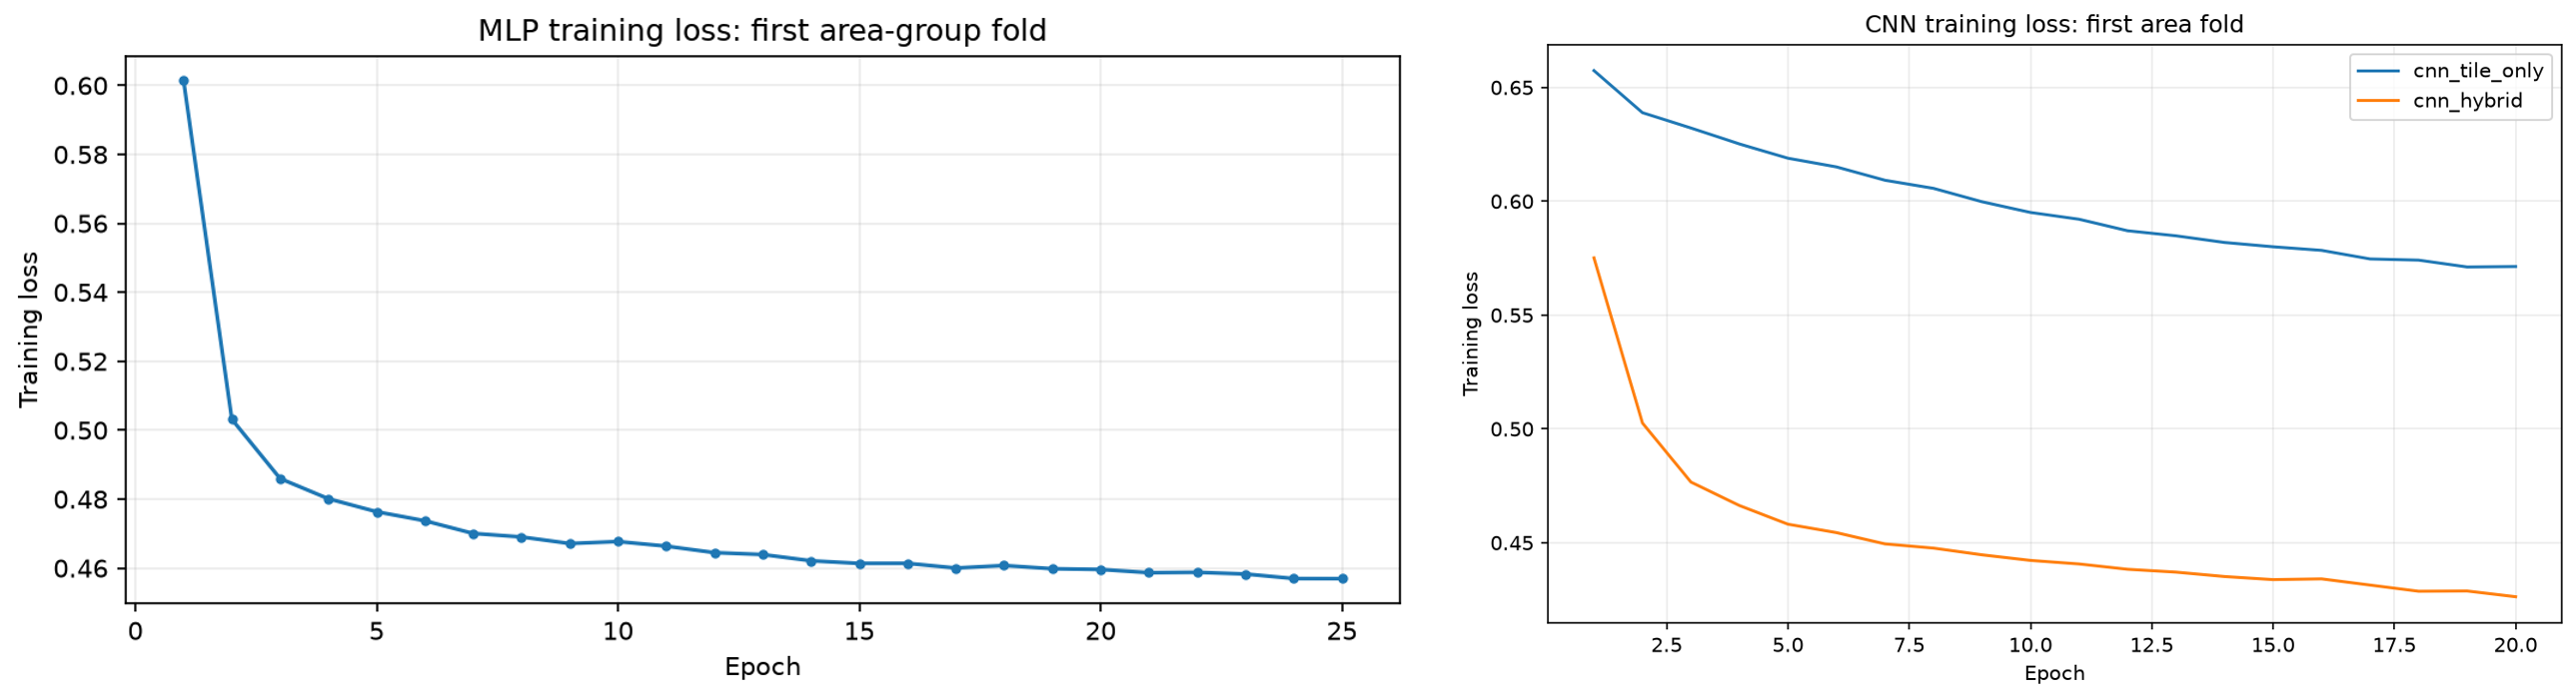
\includegraphics[width=0.92\linewidth]{figures/training_loss.png}
\caption{Training loss (binary cross-entropy) on the first area-group fold. Left: MLP. Right: image-only CNN (blue) and hybrid CNN (orange).}
\label{fig:loss}
\end{figure}

\subsection{One-time test on an unseen storm (Imelda 2019)}
Table~\ref{tab:test} shows the frozen final models on Imelda. LightGBM is best on every metric: it detects 86.6\% of reported flood locations at 79.8\% precision, with accuracy 0.820 and ROC-AUC 0.890, close to its validation scores, so it transfers to a later storm with a very different rainfall profile. \textbf{Comparison with existing studies}: Liu et al.\ \cite{liu2024interpretable} report accuracy $\approx$0.8 and true-positive rate 0.83--0.89 with tree ensembles on other U.S.\ events. Our LightGBM achieves comparable values (accuracy 0.82, TPR 0.87) on a strictly withheld future storm with only five land features. Mobley et al.\ \cite{mobley2021texas} report AUC 0.895 on insurance claims, similar to our 0.890. These studies use different labels and regions, so the comparison is indicative rather than a controlled benchmark.

\begin{table}[t]
\centering\small
\caption{One-time final test on Tropical Storm Imelda (19,164 rows) at frozen cutoffs $\tau$.}
\label{tab:test}
\begin{tabular}{lcccccccc}
\toprule
Model & $\tau$ & Accuracy & Precision & Recall & F1 & ROC-AUC & PR-AUC \\
\midrule
Dummy (reference) & .50 & .509 & .509 & 1.000 & .674 & .500 & .509 \\
Logistic regression & .44 & .695 & .663 & .813 & .730 & .751 & .717 \\
MLP & .47 & .769 & .740 & .840 & .787 & .843 & .812 \\
CNN image only (experiment) & .38 & .683 & .638 & \textbf{.871} & .737 & .768 & .748 \\
CNN hybrid & .47 & .795 & .773 & .846 & .808 & .875 & .853 \\
\textbf{LightGBM} & .50 & \textbf{.820} & \textbf{.798} & .866 & \textbf{.830} & \textbf{.890} & \textbf{.860} \\
\bottomrule
\end{tabular}
\end{table}

\subsection{Ablation studies}
\textbf{Rainfall (feature ablation).} Every tabular model was trained with and without event rainfall (Fig.~\ref{fig:rain}). Within the area-group design rainfall helps slightly (LightGBM ROC-AUC 0.901 vs.\ 0.891), but for new storms it is harmful. LightGBM's LOSO recall falls from 0.884 to 0.483 and ROC-AUC from 0.902 to 0.828, with similar collapses for RF, XGBoost and the MLP. Trees cannot extrapolate beyond the rainfall range of the training storms: for flooded Harvey locations, out-of-fold scores \emph{decreased} as rainfall increased (mean 0.41 for 8--11~in.\ to 0.16 for 17--21~in.). Rainfall was therefore excluded from all final models. This decision was made before the Imelda test.

\begin{figure}[t]
\centering
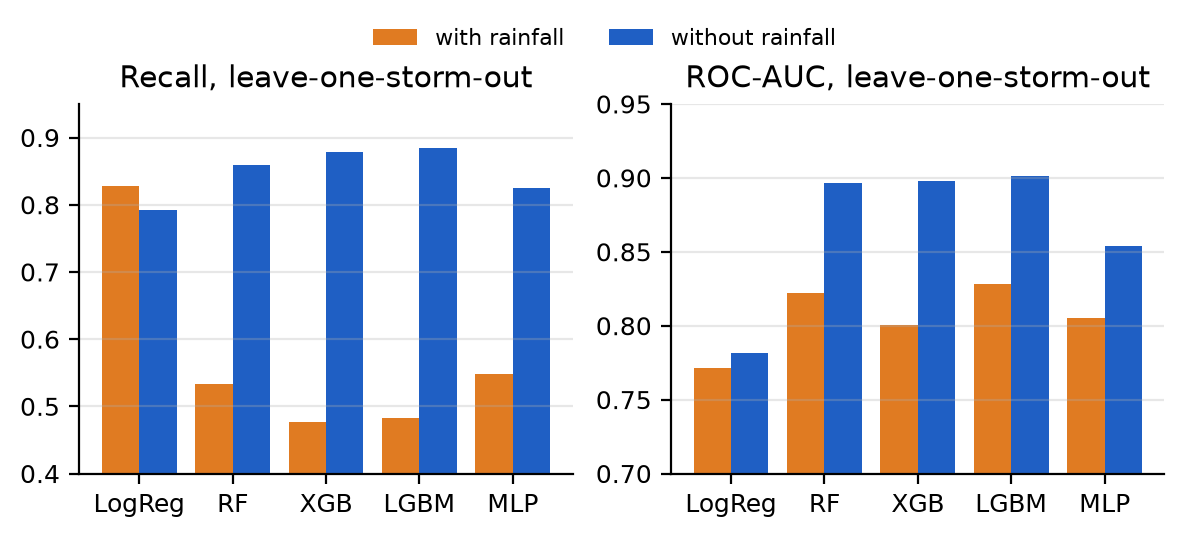
\includegraphics[width=0.9\linewidth]{figures/rain_ablation.png}
\caption{Rainfall ablation under leave-one-storm-out validation. Including event rainfall sharply reduces recall and ROC-AUC on held-out storms for all non-linear models.}
\label{fig:rain}
\end{figure}

\textbf{Hyperparameters.} A RandomizedSearchCV over seven LightGBM hyperparameters (trees 100--500, learning rate 0.01--0.1, leaves 15--63, depth, minimum child samples and two regularisers: 2,916 combinations, 20 sampled per search, optimising ROC-AUC) inside nested CV did \emph{not} improve any of the 12 average metrics (e.g.\ ROC-AUC 0.891$\to$0.889 for new places and 0.902$\to$0.898 for new storms). Only 1 of 8 outer folds improved, by 0.0003. The default setting is already well regularised for five features, so the extra search mainly adds variance.

\textbf{Input modality and network depth/width.} Terrain images alone (CNN image only) lose 0.11--0.13 ROC-AUC against tabular LightGBM, and adding the tabular features to the CNN (hybrid) recovers most of the gap. Model capacity matters less than inductive bias. The 2.7k-parameter MLP and the 28k-parameter hybrid CNN both stay below 300 boosted trees on these features.

\textbf{Cutoff transfer.} Choosing $\tau$ on area folds and applying it unchanged to new storms works for the no-rainfall models (LightGBM LOSO recall 0.884 at $\tau$=0.50). For the rainfall models it fails (recall 0.46 at their area-selected cutoff of 0.51), which is another symptom of the shift.

\subsection{Explanations and repeat flooding}
Mean $|$SHAP$|$ (Fig.~\ref{fig:shap}a) ranks elevation first (1.33 log-odds), then highway proximity (0.72) and slope (0.65), with land cover and distance to bayou contributing less. Low, flat, highway-adjacent land looks most like past flood locations, which is consistent with Liu et al.'s finding that hydrological and topographic features dominate \cite{liu2024interpretable}. SHAP describes what the model uses, not causation. As an external sanity check (Fig.~\ref{fig:shap}b), 928 grid cells had 311 reports in all four storms, and the model's mean score increases monotonically with the number of storms in which a cell flooded (0.11, 0.21, 0.36, 0.48, 0.66), although the model never sees flood frequency. The scores come from the final model trained on 2015--2017, so three of the four storms are in-sample for this check.

\begin{figure}[t]
\centering
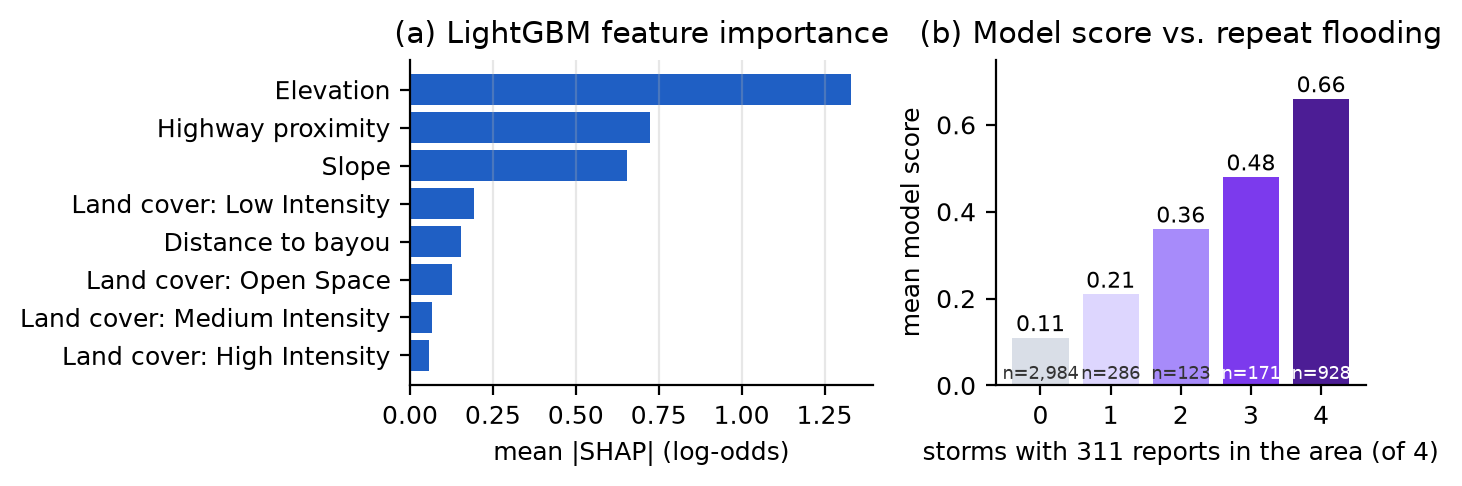
\includegraphics[width=0.95\linewidth]{figures/shap_repeat.png}
\caption{(a) Global LightGBM feature importance (mean $|$SHAP$|$, 5,000 training rows). (b) Mean model score of grid cells by the number of storms (of 4) with 311 reports in the cell.}
\label{fig:shap}
\end{figure}

\subsection{Computational complexity}
Table~\ref{tab:cost} summarises cost on a 12-core Intel laptop CPU without a GPU. Building the terrain images was the most expensive step: reprojecting 76 one-metre DEM tiles and extracting 66,514 windows took 2.26~h, and the training tile array occupies 136~MB in float16. The final LightGBM trains on all 66,514 rows in 0.76~s, scores 19,164 locations in 64~ms (3.4~$\mu$s per location) and serialises to about 1~MB. The CNNs cost about 1.2~M multiply-accumulates per image and three orders of magnitude more training time for lower accuracy.

\begin{table}[t]
\centering\small
\caption{Model size and cost. Times are wall-clock on CPU. Validation time covers all 8 folds (5 area + 3 storm).}
\label{tab:cost}
\begin{tabular}{lrrr}
\toprule
Model & Parameters & Inference cost / sample & Validation time \\
\midrule
Logistic regression & 9 & 9 MACs & -- \\
Random forest & 300 trees & 300 tree traversals & 32.6 s \\
XGBoost & 300 trees (depth $\le$6) & 300 traversals & 7.3 s \\
LightGBM (final) & 300 trees ($\le$31 leaves) & 3.4 $\mu$s measured & 6.6 s \\
MLP & 2,689 & 2.6 k MACs & 209.7 s \\
CNN image only & 23,361 & 1.20 M MACs & 41.3 min \\
CNN hybrid & 28,033 & 1.21 M MACs & 34.2 min \\
\bottomrule
\end{tabular}
\end{table}

\subsection{Challenges and solutions}
\begin{itemize}
\item \textbf{Misaligned sources} (different coordinate systems and resolutions): all layers reprojected to UTM 15N, with one value looked up per location.
\item \textbf{Very large rasters} ($\sim$93~GB listed): only the 76 tiles covering samples were downloaded; windowed $32\times32$ extraction with float16 storage; a timed two-tile pilot came before the full 2.26~h build.
\item \textbf{Noisy 311 labels}: flood categories were filtered, duplicates merged, and the label scope documented as \emph{reported} flooding.
\item \textbf{Spatial and temporal leakage}: grouped CV by grid cell, LOSO, fold-local preprocessing, and frozen cutoffs plus a locked one-time test.
\item \textbf{Rainfall shift}: diagnosed with LOSO and Harvey rainfall bins, then removed before testing.
\item \textbf{Communicating results}: SHAP values are turned into plain-language sentences in a public map.
\end{itemize}

\subsection{Deployment: FloodSense 2.0}
The frozen LightGBM scores and SHAP values for 62,138 sampled locations are aggregated to the 4,492 grid cells and served as a static web map (\url{https://floodsense-2.netlify.app}). Users can explore the susceptibility surface, overlay each storm's 311 reports, inspect a street with a per-area explanation, and view the repeat-flooding areas (Appendix~\ref{app:app}).

%=====================================================================
\section{Conclusion}
%=====================================================================
We framed Houston flood-hotspot identification as an explainable classification problem over fused geospatial data and evaluated it under protocols that prevent spatial and temporal leakage. Five land features with LightGBM detect 87\% of reported flood locations at 80\% precision on a storm withheld until the end, matching prior work on a harder, strictly unseen test, at negligible cost. Negative results are equally informative: event rainfall hurts cross-storm transfer, tuning brings no gain, and terrain-image CNNs do not beat tabular trees. \textbf{Limitations}: 311 reports miss unreported flooding and reflect who calls the city; negatives are sampled, so scores are relative susceptibility, not probabilities of flooding; the test covers one storm whose locations largely overlap the training cells; and the map is not a forecast. \textbf{Future work}: more storms and cities, positive-unlabelled learning for missing reports, drainage-network and impervious-surface features, and event-aware models that can use rainfall without breaking transfer.

\bibliographystyle{plain}
\bibliography{refs}

%=====================================================================
\appendix
\section{Full validation results including rainfall variants}
\begin{table}[h]
\centering\small
\caption{Mean validation scores with rainfall (default cutoff 0.5). Compare with Table~\ref{tab:val}.}
\begin{tabular}{l ccc ccc}
\toprule
 & \multicolumn{3}{c}{Area-group CV} & \multicolumn{3}{c}{Leave-one-storm-out}\\
\cmidrule(lr){2-4}\cmidrule(lr){5-7}
Model (with rainfall) & Recall & F1 & ROC-AUC & Recall & F1 & ROC-AUC\\
\midrule
Logistic regression & .789 & .745 & .784 & .827 & .741 & .771\\
Random forest & .824 & .817 & .887 & .533 & .608 & .822\\
XGBoost & .857 & .834 & .900 & .477 & .526 & .800\\
LightGBM & .858 & .835 & .901 & .483 & .551 & .828\\
MLP & .832 & .797 & .862 & .548 & .564 & .805\\
\bottomrule
\end{tabular}
\end{table}

\section{Hyperparameter search space}
\begin{table}[h]
\centering\small
\caption{LightGBM nested randomized search (20 configurations per outer fold, ROC-AUC, seed 42).}
\begin{tabular}{ll}
\toprule
Hyperparameter & Candidate values\\
\midrule
n\_estimators & 100, 200, 300, 500\\
learning\_rate & 0.01, 0.05, 0.1\\
num\_leaves & 15, 31, 63\\
max\_depth & 5, 10, $-1$\\
min\_child\_samples & 20, 50, 100\\
reg\_alpha, reg\_lambda & 0, 0.1, 1\\
\bottomrule
\end{tabular}
\end{table}

\section{CNN inputs}
\begin{figure}[h]
\centering
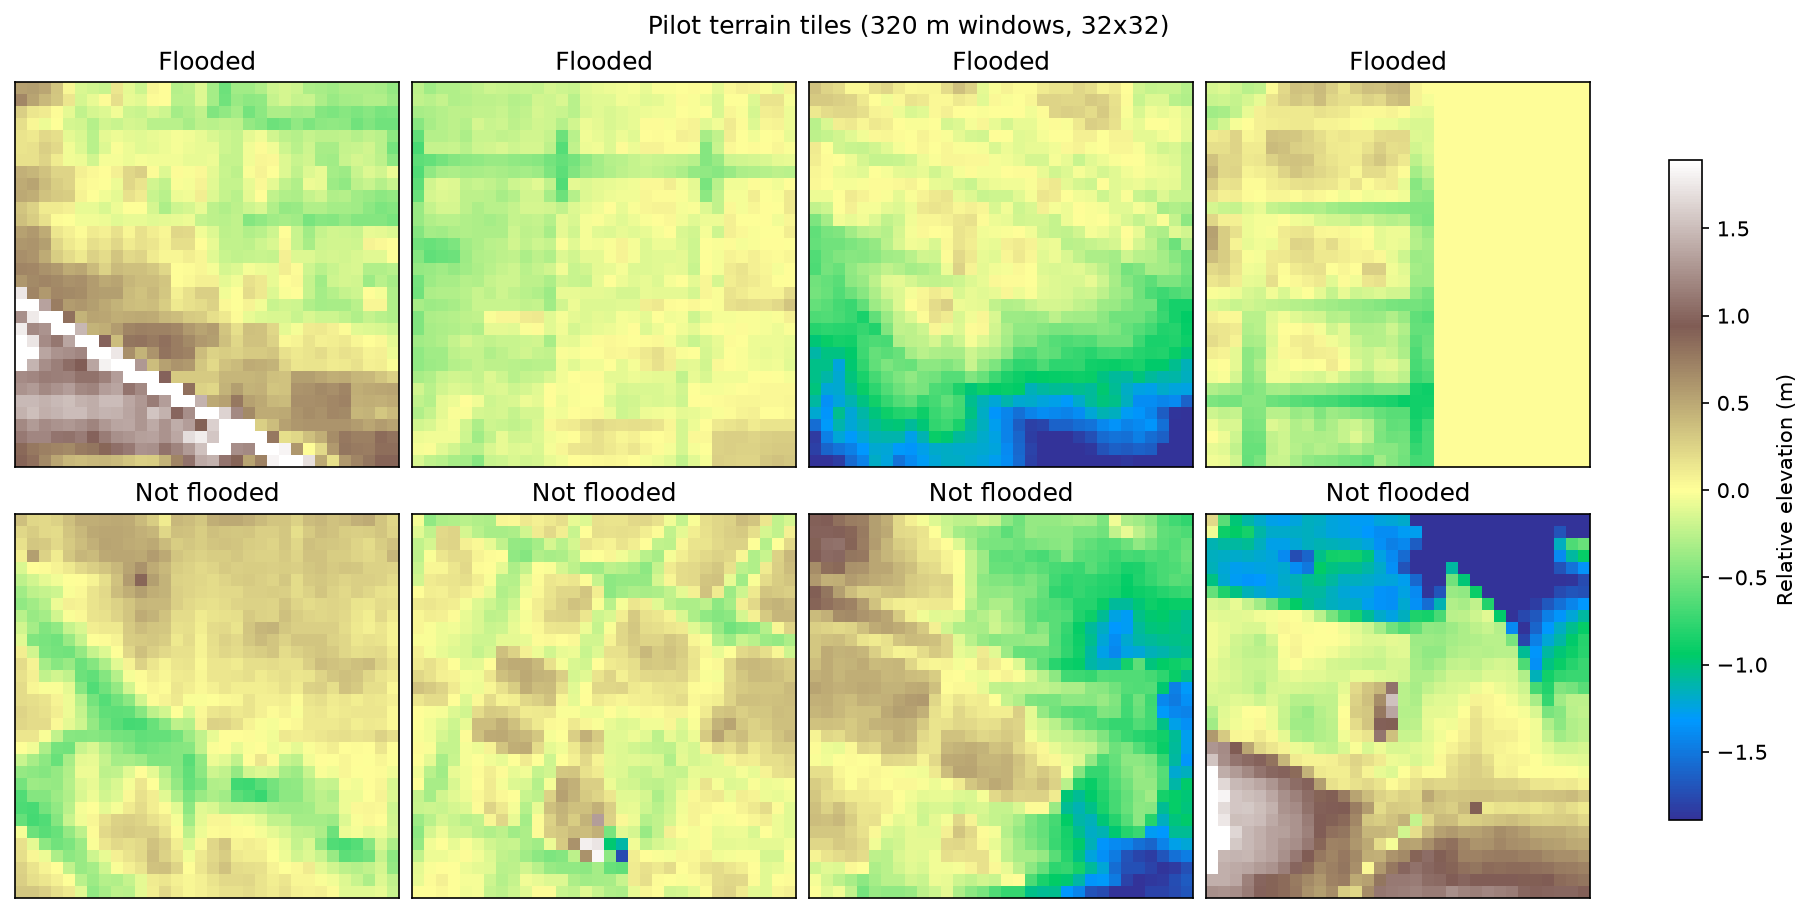
\includegraphics[width=0.85\linewidth]{figures/example_tiles.png}
\caption{Example $32\times32$ relative-elevation training tiles (320~m) for flooded and not-flooded locations.}
\end{figure}

\section{FloodSense 2.0 application}\label{app:app}
\begin{figure}[h]
\centering
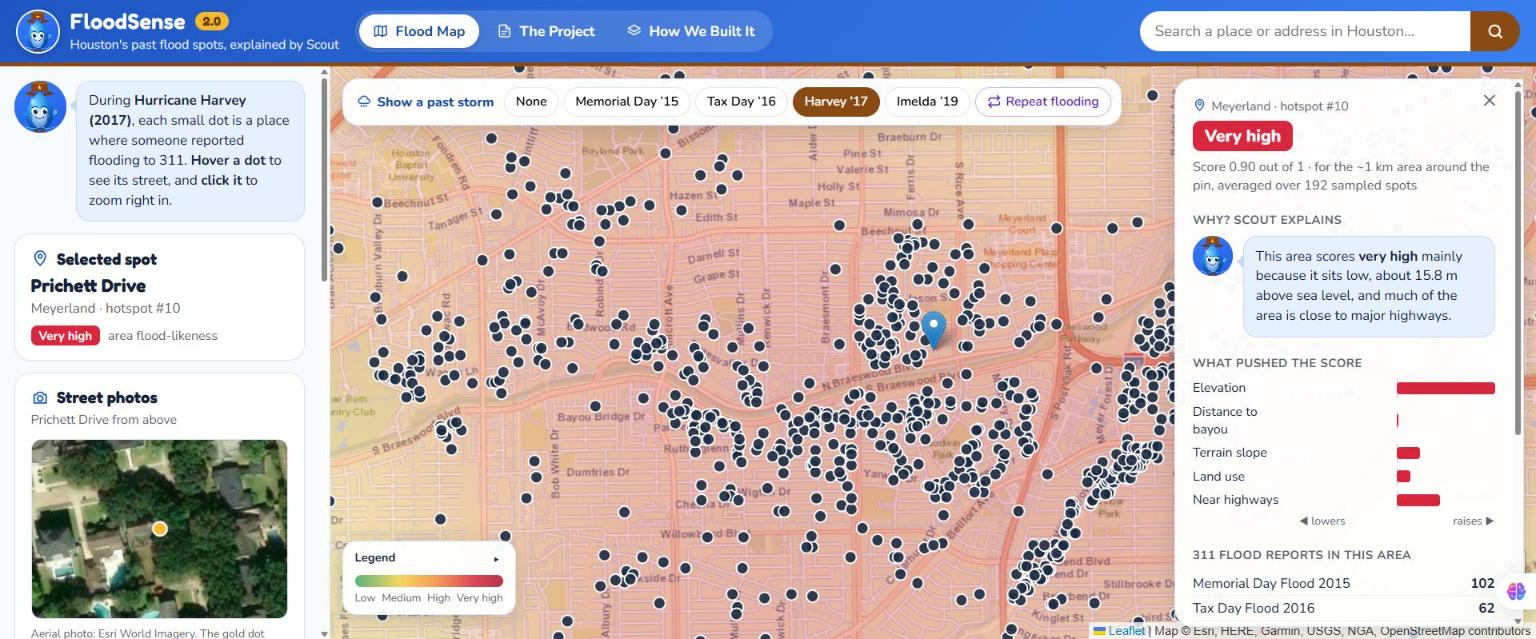
\includegraphics[width=\linewidth]{figures/app_harvey.jpg}
\caption{FloodSense 2.0 during Hurricane Harvey: 311 reports (dots) over the susceptibility surface; the card explains a ``Very high'' area in plain language from its SHAP values.}
\end{figure}

\section{Reproducibility}
Code, notebooks (01\_data\_cleaning to 12\_shap and the tuning notebook), frozen setup, saved results and figures are in the project repository (\texttt{reports/}, \texttt{docs/}). The report's figures are regenerated by \texttt{report/make\_figures.py} from the saved results, without retraining.

\end{document}
